% 1992 年上海卷第 10 题：直平行六面体 A₁C，上底面 ABCD 为菱形，E 为 A₁B₁ 中点，F 为 AA₁ 中点，M 为 AC 与 BD 的交点
% 依固定扫描页重绘，只画拓扑与标号，不按比例
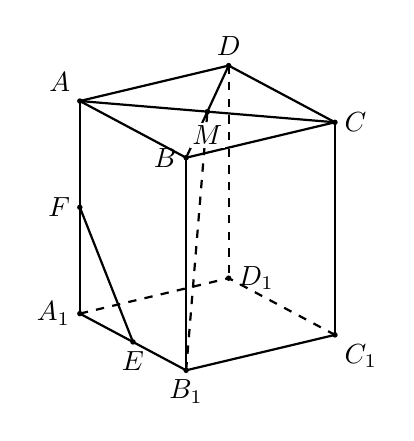
\begin{tikzpicture}[>=stealth,scale=0.9,line join=round]
  % 上底面 ABCD
  \coordinate (A) at (-2,0.9);
  \coordinate (B) at (-0.5,0.1);
  \coordinate (C) at (1.6,0.6);
  \coordinate (D) at (0.1,1.4);
  % 下底面 A1B1C1D1（向下平移）
  \coordinate (A1) at (-2,-2.1);
  \coordinate (B1) at (-0.5,-2.9);
  \coordinate (C1) at (1.6,-2.4);
  \coordinate (D1) at (0.1,-1.6);
  \coordinate (M) at (-0.2,0.75);
  \coordinate (E) at (-1.25,-2.5);
  \coordinate (F) at (-2,-0.6);

  % 可见棱
  \draw[thick] (A)--(B)--(C)--(D)--cycle;
  \draw[thick] (A)--(A1);
  \draw[thick] (B)--(B1);
  \draw[thick] (C)--(C1);
  \draw[thick] (A1)--(B1)--(C1);
  % 不可见棱
  \draw[thick,dashed] (A1)--(D1)--(C1);
  \draw[thick,dashed] (D)--(D1);
  % 上底面对角线 AC、BD 与交点 M
  \draw[thick] (A)--(C);
  \draw[thick] (B)--(D);
  % EF
  \draw[thick] (E)--(F);
  \draw[thick,dashed] (B1)--(M);

  \fill (A) circle (1.1pt) node[above left] {$A$};
  \fill (B) circle (1.1pt) node[left] {$B$};
  \fill (C) circle (1.1pt) node[right] {$C$};
  \fill (D) circle (1.1pt) node[above] {$D$};
  \fill (A1) circle (1.1pt) node[left] {$A_{1}$};
  \fill (B1) circle (1.1pt) node[below] {$B_{1}$};
  \fill (C1) circle (1.1pt) node[below right] {$C_{1}$};
  \fill (D1) circle (1.1pt) node[right] {$D_{1}$};
  \fill (M) circle (1.1pt) node[fill=white,inner sep=1pt,below=4pt] {$M$};
  \fill (E) circle (1.1pt) node[below] {$E$};
  \fill (F) circle (1.1pt) node[left] {$F$};
\end{tikzpicture}
